\documentclass{beamer}
%\setbeamertemplate{bibliography item}{}
\usepackage[utf8]{vietnam}
\usepackage{amsmath}
\usepackage{amsfonts}
\usepackage{amssymb}
\usepackage{textpos}
\usepackage{enumerate}
\usepackage{graphicx}
%\usepackage{booktabs}
\usepackage{cite}
%\usepackage{natbib}
\usetheme{Warsaw}
\newtheorem{dn}{Định nghĩa}[section]
\newtheorem{dl}{Định lý}[section]
\newtheorem{tc}{Tính chất}[section]
\newtheorem{hq}{Hệ quả}[section]
\newtheorem{bd}{Bổ đề}[section]
\newtheorem{md}{Mệnh đề}[section]
\newtheorem{vd}{Ví dụ}[section]
\newtheorem{nx}{Nhận xét}[section]
\newcommand{\dom}{\text{{\rm dom}}}
\newcommand{\epi}{\text{{\rm epi}}}
\newcommand{\Min}{\text{{\rm Min}}}
\setbeamertemplate{theorems}[numbered]
\setbeamertemplate{definitions}[numbered]
\setbeamertemplate{footline}[frame number]
\usepackage{algorithm}
\usepackage{color}
\usepackage{algorithmic}
\usepackage{footmisc}
%\usepackage{enumitem}
\usepackage{indentfirst} 
\usepackage{comment}
\renewcommand{\thefootnote}{\arabic{footnote}}
\usefonttheme{professionalfonts}
\setbeamercolor{normal text}{bg=white,fg=black}
\renewcommand{\thefootnote}{\arabic{footnote}}
%kt
\mode<presentation>
{
 \usetheme{Darmstadt}
%\usetheme{Rochester}
}
\beamertemplatetransparentcoveredhigh

\begin{document}
\title[]{\fontsize{13pt}{10pt}\selectfont {\bf \LARGE   Phương pháp giải bài toán \\Tối ưu tuyến tính chứa tham số}\\
------------------------------------------

{\small Hướng dẫn: PGS.TS. Tạ Quang Sơn}} 
\author[]{\bf Thực hiện : NGUYỄN THÀNH NAM \& LÊ ĐỨC ANH \\
Sinh viên lớp: DTU1221, Khóa: 22}
\institute[Báo cáo luận văn thạc sĩ]{\fontsize{2pt}{2pt}}%
\small{\date{\today}}
\begin{frame}
\begin{center}
{\fontsize{8pt}{8pt}\selectfont \bf{ỦY BAN NHÂN DÂN THÀNH PHỐ HỒ CHÍ MINH\\
TRƯỜNG ĐẠI HỌC SÀI GÒN}}
\end{center}
\begin{center}
\end{center}

\begin{center}
{\fontsize{10pt}{6pt}\selectfont \bf{BÁO CÁO ĐỀ CƯƠNG NGHIÊN CỨU KHOA HỌC\\
NGÀNH: TOÁN ỨNG DỤNG}}
\end{center}
\titlepage
\end{frame}
\begin{frame}
    \frametitle{NỘI DUNG BÁO CÁO}
    \tableofcontents
\end{frame}

\section{Mục đích nghiên cứu}

\begin{frame}{\bf Mục đích nghiên cứu}
    $\bullet$ Quy hoạch tuyến tính là một môn học trong chương trình đào tạo Cử nhân Toán ứng dụng. Lý thuyết về các phương pháp giải bài toán tối ưu tuyến tính đã được giới thiệu.
    
    \medskip
    $\bullet$ Quy hoạch tuyến tính có nhiều ứng dụng trong các bài toán kinh tế. Các bài toán ấy có thể mô hình hóa dưới dạng:
 $$
\begin{array}{cl}
{\rm Max \,(Min)} & \langle c,x \rangle\\
{\rm s.t.}& Ax \ge (\le)\, b,\\
& x \ge 0.  
\end{array}
$$
Trong đó, $A$ là ma trận thực cấp $m \times n$,      các véc tơ $c \in \mathbb{R}^n, b \in \mathbb{R}^m$ và $x\in \mathbb{R}^n$ là ẩn cần tìm để  tối ưu hóa hàm mục tiêu $\langle c,x \rangle$.

\medskip
    
 $\bullet$ Thực tế cho thấy rằng với một bài toán kinh tế đã xác lập xong có thể sẽ chịu những tác động khác, tức là có hiện tượng nhiễu. Đề tài nghiên cứu này  tìm hiểu  về dạng bài toán tối ưu tuyến tính có nhiễu với tên gọi  là bài toán Tối ưu tuyến tính  có chứa tham số. 
\end{frame}

\begin{frame}{\bf Một số hiện tượng nhiễu}

Qua quan sát người ta nhận thấy rằng hiện tượng nhiễu có thể xảy ra ở:
\begin{itemize}
\item Hàm mục tiêu;
\item Véc tơ hằng ở ràng buộc vế phải;
\item Hệ số gắn với từng biến.
\end{itemize}

Điều này cho thấy các vấn đề nêu trên có liên quan đến một tham số nhiễu và cần tìm hiểu tác động của tham số ấy vào mục tiêu của bài toán.



\end{frame}

\begin{frame}{Ví dụ}
$\bullet$ Bài toán tối ưu tuyến tính dưới đây có mục tiêu xác định không phù hợp (không bị chặn), cần phải điều chỉnh hàm mục tiêu.

$$
    \begin{array}{ll}            
        {\rm Min}&f(x)=-x_1+2x_2\\
            & \begin{cases}
                  x_1+x_2 \ge 1 \\
                  -x_1+x_2 \ge 1 \\
                  x_i\geq 0,\forall i=1,2.
           \end{cases} 
     \end{array}
$$

\begin{center}
\begin{figure}[ht]
 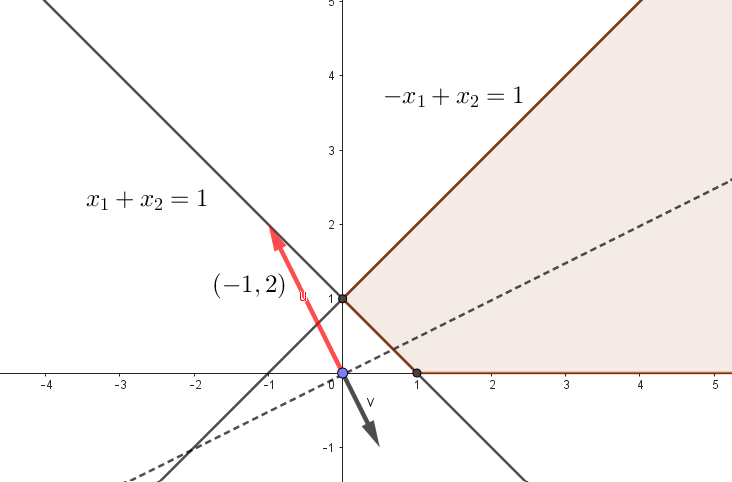
\includegraphics[width=0.50\linewidth]   {anh1vidu1.png}  
\caption{Hàm mục tiêu không bị chặn}
\end{figure}
\end{center}

\end{frame}

 

%bo



\begin{frame}
Bằng cách thay đổi hàm mục tiêu, bài toán có nghiệm.
$$
    \begin{array}{ll}            
        {\rm Min}&f(x)=x_1+2x_2\\
            & \begin{cases}
                  x_1+x_2 \ge 1 \\
                  -x_1+x_2 \ge 1 \\
                  x_i\geq 0,\forall i=1,2.
           \end{cases} 
     \end{array}
$$
\begin{center}
\begin{figure}[ht]
 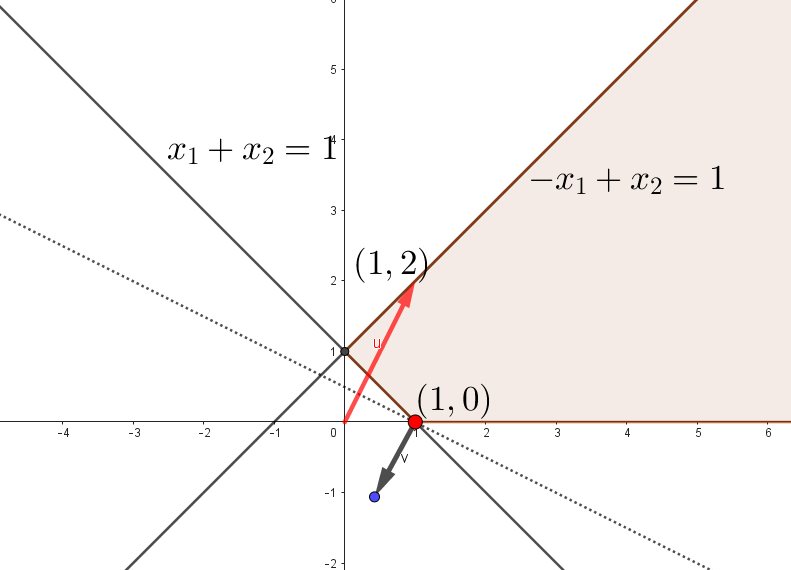
\includegraphics[width=0.5\linewidth]{anh3vidu1.png}  
\caption{Bài toán đạt tối ưu tại điểm $(1;0)$}
 \end{figure}
 \end{center}
      
\end{frame}

\begin{frame}
Thực ra việc điều chỉnh hàm mục tiêu nêu trên là kết quả của quá trình nhiễu trên hàm mục tiêu:
\begin{itemize}
\item Với véc tơ $c$ cần nhiễu
\item Xác định véc tơ nhiễu $d$
\item Với tham số nhiễu $t$, mục tiêu có nhiễu trở thành $c+td$.
\end{itemize}
\textcolor{red}{\bf Bài toán tối ưu tuyến tính có nhiễu ở hàm mục tiêu với tham số nhiễu $t$ có dạng:}
$$
    \begin{array}{lll}            
        {\rm Max (Min)}&f(x)=(c_1+td_1)x_1+\ldots+(c_n+td_n)x_n\\
            & \begin{cases}
            a_{11}x_1+\ldots+a_{1n}x_n =  b_1 \\
            \vdots\\
            a_{m1}x_1+\ldots+a_{mn}x_n =  b_m\\
            x_i\geq 0,\forall i=1,2....n
           \end{cases} 
     \end{array}
$$ 

\textcolor{red}{\bf Nếu bài toán tối ưu tuyến tính có nhiễu ở vế phải thì bằng cách chuyển qua bài toán đối ngẫu, sẽ có bài toán nhiễu ở hàm mục tiêu.}
\end{frame}



\section{Nội dung nghiên cứu}
\begin{frame}{\bf Nội dung nghiên cứu}
    \begin{itemize}
    \item Hệ thống lại cơ sở lý thuyết và phương pháp giải các bài toán Tối ưu tuyến tính.
    \item Đề tài này chọn lựa tìm hiểu về bài toán tối ưu tuyến tính có tham số thông qua 2 dạng bài toán:
    \begin{itemize}
    \item Tối ưu tuyến tính có tham số ở hàm mục tiêu.
    \item Tối ưu tuyến tính có tham số ở vế phải của ràng buộc.
    \end{itemize}
    \item Trong các trường hợp trên đề tài sẽ tìm hiểu về ảnh hưởng  của tham số tác động đến sự tồn tại nghiệm và tập nghiệm tương ứng của bài toán.
    \end{itemize}
\end{frame}
\section{Dự kiến nội dung đề tài}
\begin{frame}{\bf Dự kiến nội dung đề tài}
    \begin{itemize}
    \item Chương 1:  Bao gồm các kiến thức chuẩn bị, nội dung có liên quan đến
    một số kiến thức cơ bản của quy hoạch tuyến tính để dùng
    làm cơ sở nghiên cứu về các phương pháp giải của bài toán tối ưu tuyến tính có tham số.
    \item Chương 2: Tìm hiểu về các phương pháp và thuật giải giúp giải quyết bài toán Tối ưu tuyến tính có tham số ở hàm mục tiêu và Tối ưu tuyến tính có tham số vế phải của ràng buộc.
    \item Chương 3: Một số ví dụ áp dụng của bài toán tối ưu tuyến tính có tham số vào các bài toán cụ thể .
    \end{itemize}   
\end{frame}
\section{Tổ chức và phân công}
\begin{frame}[shrink=20]
    \frametitle{\bf Tổ chức và phân công}
    \vspace{1.5cm}
    \begin{table}
        \begin{tabular}{|p{2.5in}|c|c|}
            \hline
            \textbf{Nội dung} & Người phụ trách chính & Người cộng tác \\
            \hline \hline
            \textbf{Chương 1} && \\
            \hline
            Cơ sở lý thuyết quy hoạch tuyến tính & Nguyễn Thành Nam & \\
            & Lê Đức Anh & \\
            \hline
            \textbf{Chương 2} && \\
            \hline
           Tối ưu tuyến tính có tham số hàm mục tiêu & Nguyễn Thành Nam & Lê Đức Anh \\
           \hline
           Tối ưu tuyến tính có tham số vế phải của ràng buộc & Lê Đức Anh & Nguyễn Thành Nam\\
            \hline
            \textbf{Chương 3} && \\
            \hline
            Các bài toán ứng dụng & Nguyễn Thành Nam & \\
            & Lê Đức Anh & \\
            \hline
        \end{tabular}
    \end{table}
\end{frame}
\section{Tiến độ thực hiện}
\begin{frame}{Tiến độ thực hiện}
Thời gian nghiên cứu chia làm 3 giai đoạn:
\begin{itemize}
\item Giai đoạn 1 (? tháng): Đọc, hiểu tài liệu liên quan đến lý thuyết tối ưu tuyến tính có tham số và các phương pháp giải.
\item Giai đoạn 2 (? tháng): Thu hoạch, hệ thống lại các tri thức và viết luận văn.
\item Giai đoạn 3 (? tháng): Hoàn thành và bảo vệ luận văn.
\end{itemize}
\end{frame}


\section{Tài liệu tham khảo}

\begin{frame}{Tài liệu tham khảo}
\begin{thebibliography}{xxx}
%1%
\bibitem{T}   Tạ Quang Sơn, Bài giảng Quy hoạch tuyến tính, Đại học Sài Gòn, 2023.

\bibitem{E} Elementary Linear Programming with Applications (1995, Academic Press).

\bibitem{H} Hu T.C.-Linear and Integer Programming Made Easy.

\bibitem{L} Linear Programming - Foundations and Extensions - Springer US (2001).

\bibitem{B}Bùi Phúc Trung, Nguyễn Thị Ngọc Thanh, Vũ Thị Bích Liên, Giáo trình Quy hoạch tuyến tính Tối ưu hóa, NXB Lao Động-Xã Hội-2003

\end{thebibliography}
\end{frame}

\begin{frame}
\begin{block}{}
\medskip
\center{\huge \it \textcolor[rgb]{0.50,0.30,1.0}{Cảm ơn quý thầy cô và các anh chị đã quan tâm theo dõi!}}
\medskip
\end{block}	
\end{frame}
\end{document}

